\chapter[IYTY --- Parameter Space]{I {\em Told} You Tomorrow\\--- Parameter Space}\label{sect:discussion} 

The role of owner is very important, as he is the one who defines the value \V of the secret  and accordingly to the one of pawn \PO. The value of the secret is the entry point to determine the bids that have to be paid by the shareholders, so the bigger it is, the bigger can be the damage caused by the failure of the TL protocol.
However in general, no one but the owner can prove \V to be the right estimate of the value of a secret, and a TL is by definition a mechanism to protect it from anyone else since \td. 

Therefore, as in any real scenario, it is impossible to protect a priori the protocol against the owner's abuse, however, being the TL primitive modeled as an economic game, it is possible to prevent him to cause damages. 

The solution which we adopt is to derive the value of the pawn starting from that of the secret, specifically we impose the proportionality between the value of the secret and the pawn:

\begin{equation}\label{proprel1}
\V \propto \PO
\end{equation}

The meaning of such relation could be thought as the more \owner would like to secure, the more the exposition he has to deal with.

\section{Leveraging digital identities}
The considerations made so far stem from the fact that we do not model the existence of any reputation system, thus we found the protocol only over pure economic assumptions. An alternative could be the possibility of bounding to {\em digital wallets} the shares and the secret, leveraging their ability of punishing all those participants who behave in a malicious way.

Although it could be natural to foresee a punishing mechanism based on digital wallets, there is no easy way to exactly determine how and why a TL primitive founded on secret sharing had fail. Such a difficulty translates into the impossibility of establishing to whom the punishment must be addressed to. A clear example is the case of mixed owner-shareholder attacker coalition. If that was the case, the malicious owner could simulate an attack to the TL primitive by sending \secret to a colluded shareholder and then asking him to submit it to the smart contract. The punishment would then be automatically triggered to all honest shareholders, and the owner would be considered as the victim.

The scenario described once again makes explicit the need of simple but powerful economic constraints. As the state of TL protocol failure can be reached only by the submission of \secret (the proof of possession), then the owner will be careful in its management before \td, since its submission entails the lost of his pawn, whose value we remind to be proportional to \secret, as said in relation~\ref{proprel1}.

Also we highlight that foreseeing a reward to the owner might look as the requirement of him to assume an active role at disclosure time, but this is not true because, as already said, the owner reward only ensures him to keep his interest into the secret. This settle makes our solution particularly suitable in scenarios in which the owner goes offline for indeterminate periods of time and then comes back online to get his reward back, for example in the context of proof of retrievability services.

Anyway, the assumption of the availability of reputation control systems would anyway have a heavy impact over our model, limiting the role of the owner to the activation time, and thus would simplifying equality~\ref{eqbalance4} and proportionality relation~\ref{proprel1}.

\section{Evaluating trust}

Before participating to a TL protocol, a shareholder may want to evaluate the conditions offered by the owner. The parameters that have been introduced so far permits only to evaluate the profit (\profit) and the approximate instant of time (\td) at which it will materialize, yet this information is not enough for \shareholder to decide whether to participate or not.
In order to perform an exhaustive evaluation, the shareholder needs some additional feedback information about both the availability of the system and the will of the owner. 

The availability of the system can be thought as something close to the expectation of a TL protocol to be successful, in other words, a measure of the {\em trust on the system}, to which we address to with $\Phi \left( t \right)$. 
If we rewrite relation~\ref{proprel1} making clear the proportionality by the time dependent coefficient $\phi \left( t \right) > 0$ , so that:
\begin{equation}\label{proprel2}
\PO = \phi \left( t \right) \cdot \V
\end{equation} 
we obtain an the indicator, $\phi \left( t \right)$, whose performance is closely correlated to the one of $\Phi \left( t \right)$. The idea is that the more $\phi \left( t \right)$ will be close to zero the more the system will be trustful, so a shareholder might be inclined to accept an owner to deposit low pawns. On the contrary, the more $\phi \left( t \right)$ will grow, the less a shareholder might be inclined to accept a TL primitive with low owner pawn. 

In order to represent the will of the owner, another indicator could be introduced, more specifically, the magnitude of the {\em distance} between the owner and the role of whistleblower. Such an indicator can be expressed as:
\begin{equation}\label{proprel3}
\xi = \frac{\RO - \Wbonus}{\RO}
\end{equation} 
whose value ranges from 0 to 1. The more the distance will be close to 0, the more notable the promise of \owner to not break the TL primitive (the bigger his will to keep interest into \secret), the more the distance will be close to 1 the less the owner will behave reliably. 


\section{Security without losing replication}

\begin{figure}[t]
	\centering
	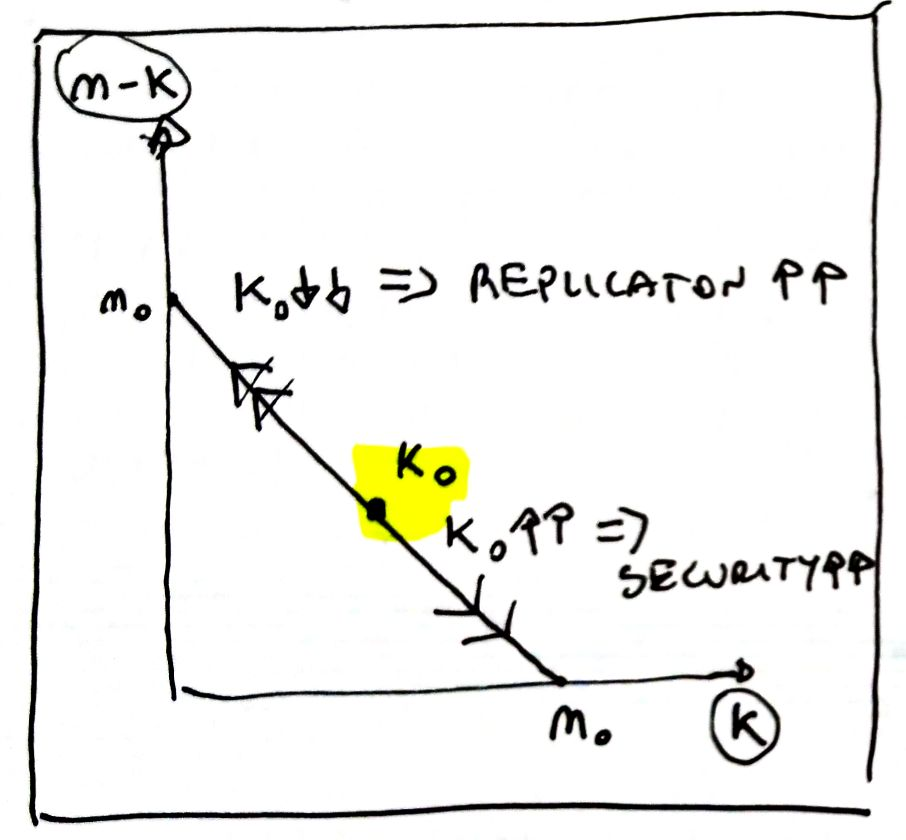
\includegraphics[width=.5\textwidth]{fig/rse_a}
	\caption{Replication and security in Shamir's Secret Sharing}
	\label{fig:rsea}
\end{figure}

\begin{figure}[t]
	\centering
	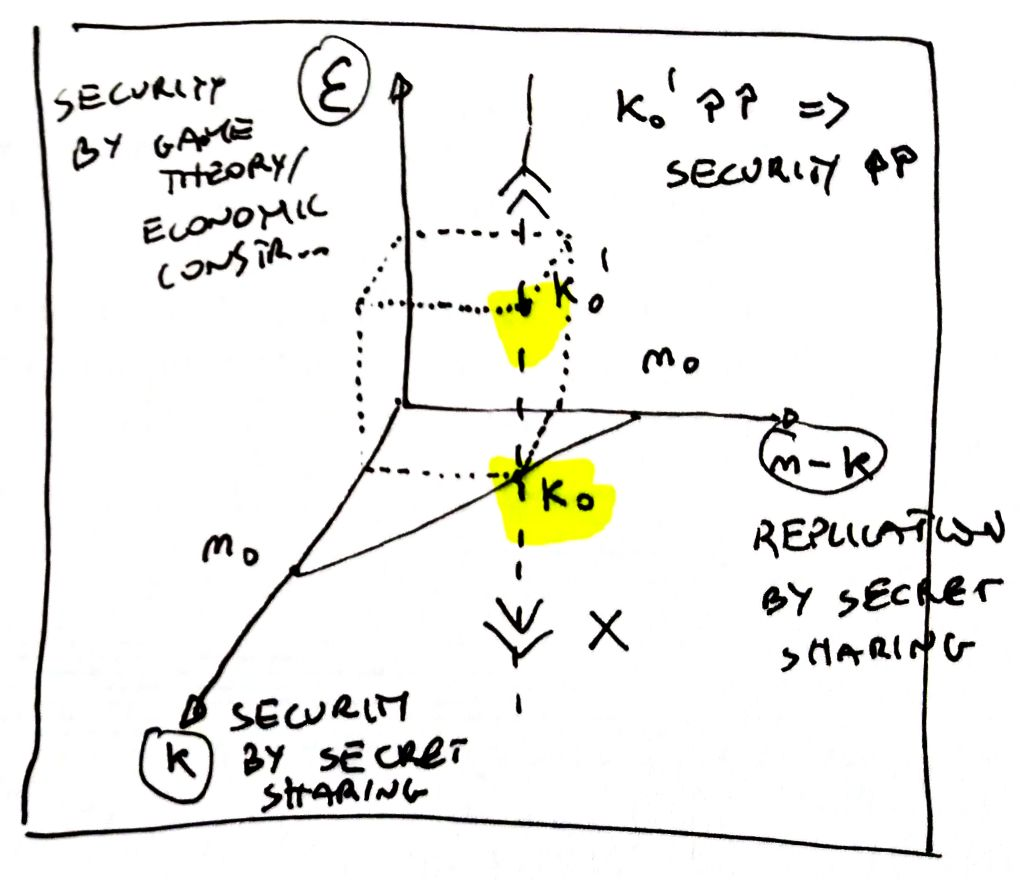
\includegraphics[width=.55\textwidth]{fig/rse_b}
	\caption{Replication and security in \shortname}
	\label{fig:rseb}
\end{figure}


\begin{algorithm}[t]
	\SetKwFunction{Assert}{assert}
	\SetKwInOut{Input}{input}
	\SetKwInOut{Output}{output}
	\SetKwFunction{FMain}{compute\textunderscore params}
	\SetKwProg{Fn}{Function}{}{}
	
	\BlankLine
	\Input{
		\V value of the secret \\
		\N number of shareholders \\
		\K Shamir threshold \\
		\lost number of compromised shareholders \\
		$\phi$ trust on the system evaluator \\
		\profit shareholder's profit \\
		\extrareward reconstruction extra profit \\
		$\xi$ owner distance \\
		$\epsilon$ reconstruction exposure
	}
	
	\BlankLine
	\Output{
		\PO owner pawn \\
		\RO owner reward \\
		\RH shareholder reward \\
		\BH shareholder bid \\
		\Wbonus whistleblowing bonus
	}
	
	\BlankLine
	\Fn{\FMain{$\V, \N, \K, \lost, \phi, \profit, \extrareward, \xi, \epsilon$}}{
		{$\PO \leftarrow \phi \cdot \V$} \\
		{$\RO \leftarrow \PO - \N \cdot \profit - \K \cdot \extrareward$} \\
		\Assert{$\RO > 0$, "non satisfiable economic conditions"}
		
		\BlankLine
		{$\Wbonus \leftarrow \RO - \xi \cdot \RO$}
		
		{$\BH_{0} \leftarrow \left( \V + \Wbonus \right) / \left( \K - \lost \right)$} \\
		{$\BH_{1} \leftarrow \V / \left( \N - \K - \lost + 1 \right)$} \\
		\Assert{$\BH_{0} > 0$, "n-k-rho parameterization"} \\
		\Assert{$\BH_{1} > 0$, "n-k-rho parameterization"}
		
		\BlankLine
		{$\BH \leftarrow max \left( \BH_{0},\ \BH_{1} \right)$} \\
		{$\RH \leftarrow \BH + \profit $} \\
		\Assert{$\Wbonus > \RH $, "unfeasible whistleblowing"}
		
		\BlankLine
		\KwRet$ \left( \PO,\ \RO,\ \RH,\ \BH,\ \Wbonus \right)$
	}
	
	
	\caption{Economic parameters configuration}\label{algo_params}
\end{algorithm}

Traditional secret sharing cryptographic schemes allow to sharing a secret among a group of peers and avoiding its reconstruction until a sufficiently large group of them does not reach consensus. As already described in the previous sections, not all the possible groups can reconstruct the secret, but only the ones who satisfy the condition of threshold reach. 

The user, in this case the owner, can then leverage the parameter \K in order to set the threshold to the desired value: an increase of it would imply a stronger security but a weaker replication level, while the reduction of it the opposite. Therefore \owner, as shown in figure~\ref{fig:rsea}, can not act simultaneously on both security and replication, as the increase of one entails the reduction of the other.

Although \shortname is built on the Shamir secret sharing scheme, it allows the owner to tune replication and security simultaneously, specifically the security requirement can be achieved leveraging economic nature of the protocol. Given \K as the threshold value in order to get the proper level of replication, then the owner sets the value \BH, which he claims to be appropriate to protect the secret whose value he believes to be \V. Doing so, \owner can ask the shareholders to be more exposed in order to get the shares, and the more exposition they have to deal with, the more they will be interested in the success of the protocol. 

To capture the previous considerations we define the {\em reconstruction exposure} as a property related to the possible coalition of malicious attackers, so starting from inequality~\ref{eqcoscom3}, it follows:
\begin{equation}\label{eqtotexp}
\epsilon = (\K - \lost) \cdot \BH - \V - \Wbonus > 0
\end{equation}
The effect of the {\em reconstruction exposure} is shown in the figure~\ref{fig:rseb}, while a function to easily compute all the economic parameters is shown in algorithm~\ref{algo_params}.
